\documentclass[11pt, oneside]{article}   	% use "amsart" instead of "article" for AMSLaTeX format
\usepackage[margin=0.75in]{geometry}                		% See geometry.pdf to learn the layout options. There are lots.
\geometry{letterpaper}                   		% ... or a4paper or a5paper or ... 
%\geometry{landscape}                		% Activate for rotated page geometry
%\usepackage[parfill]{parskip}    		% Activate to begin paragraphs with an empty line rather than an indent
\usepackage{graphicx}				% Use pdf, png, jpg, or eps§ with pdflatex; use eps in DVI mode
								% TeX will automatically convert eps --> pdf in pdflatex		
\usepackage{amssymb}
\usepackage{hyperref}

\usepackage{color}
\usepackage{subcaption}
\usepackage{caption}
\usepackage[margin=10pt,font=small,labelfont=bf,
labelsep=endash]{caption}


\newcommand{\todo}[1]{ \textcolor{red}{\bf{To Do:} #1}}
\newcommand{\toref}[1]{ \textcolor{blue}{\bf{REFERENCE #1}}}
\newcommand{\future}[1]{ \textcolor{green}{\bf{Future Direction: #1}}}

%SetFonts

%SetFonts


\title{9 Month TAP Report}
\author{Me :)}
\date{}							% Activate to display a given date or no date

\begin{document}
\maketitle

\section{Low Temperature Plasmas and Wound Healing}
Wounds and their management present an issue, both in the UK and globally \cite{Posnett2008the}.
In particular, chronic wounds present a significant socio-economic burden, with 1-2 \% of the population of developed countries expected to develop a chronic wound during their lifetime \cite{Siddiqui2010chronic}, and the estimated cost of wounds to the national health service (NHS) in 2012/13 was �5 billion \cite{Guest2015health}.
Alongside this, chronic wounds can have a significant detrimental effect on the mental health of patients, for example, due to pain, odour, mobility issues and stress as a direct result of having a chronic wound \cite{Persoon2004leg}.
New wound treatment strategies are being sought, with aims to acclerate the wound healing process to decrease the risk of infection and to decrease the bacterial load in the wound. One technique under investigation is low temperature plasma (LTP), which has shown promise for both reducing the bacterial load in a wound and promoting the healing process \cite{Kong2009plasma, Kramer2013suitability, Isbary2012successful, Isbary2010a}.

Low temperature plasmas (LTP) are weakly ionised plasmas, existing far from thermodynamic equilibrium.
This results in a plasma that has an overall temperature of $\approx$ 25-40$^\circ$C, which can be applied to biological samples without causing thermal damage. 
Evidence for the successful use of LTP in wound healing comes from both laboratory experiments and clinical trials.
For example, the ability of LTP to enhance keratinocyte migration and proliferation in scratch test assays has been demonstrated in the laboratory \cite{Tipa2011plasma}, and clinically, devices such as KinPen and MicroPlaSter have shown promise when used on human patients, aiding healing without any obvious side-effects \cite{Isbary2013cold, Isbary2012successful, Isbary2010a, Bekeschus2016the}.

For the proposed mechanism of action for LTPs in both wound healing promotion and bacterial killing, please refer to my 6 month TAP report.


\subsection{Project Aims}
The overall aims of the project are to investigate the use of low temperature air plasma for wound healing applications. In particular:
\begin{enumerate}
\item Develop an air plasma source that is suitable for optical diagnostics \& treatment of biological samples
\item Characterise the plasma using optical diagnostic techniques to determine species densities, alongside the use of a global model, which will help with species densities predictions and guiding of experiments
\item Develop experiments to determine the effects of low temperature air plasma on biological samples \textit{in vitro}, for example, oxidative stress induction and wound healing promotion. Using these experiments, the difference in biological effects when plasma parameters (and, therefore, plasma composition) are changed can be investigated.
\end{enumerate}


\section{Work to Date}
\subsection{Simulations}
In the last few months I have been continuing with plasma simulations, in particular, the development of a comprehensive nitrogen chemistry set for use in GlobalKin.
GlobalKin is a global plasma chemistry model that calculated time evolved species densities given plasma power, geometry and feed gas, as shown in \textbf{figure \ref{fig:GlobalKin}} \cite{Stafford2004O2}.
For detailed information on this model, please refer to my 3 and 6 month TAP reports.

In the last TAP meeting I presented the nitrogen chemistry, with its 31 species and over 200 reactions including electron impact reactions, heavy particle reactions and vibrational kinetics.
I also highlighted areas for improvement, in particular, vibration-vibration (V-V) and vibration-translation (V-T) reactions and rates.
This is what I will discuss next.

\begin{figure}
\centering
\includegraphics[width=0.7\textwidth]{Figures/GlobalKin}
\caption{Diagram outlining how GlobalKin works. Firstly, ODEs for species density and electron temperature are constructed. This takes direct GlobalKin inputs specified by the user, as well as electron reaction rate coefficients, diffusion coefficients and mobilities from the Boltzmann solver. An ODE solver then solves the equations and the new species densities are fed back into the ODEs and Boltzmann solver, for new densities to be calculated. At regular intervals, the Boltzmann solver also updates and new coefficients are fed back into the ODEs for the ODE solver to work with. This results in the time evolution of species densities and electron temperatures.}
\label{fig:GlobalKin}
\end{figure}


\subsection{Vibration-vibration reactions in nitrogen plasmas}

As mentioned previously, vibrational kinetics are important to include in plasma chemistries, due to their influence on the electron energy distribution function (EEDF) through population of vibrationally excited states by electron impact (\textbf{equation \ref{eqn:ElectronVibration}}: and superelastic collisions between electrons and vibrationally excited states (whereby electrons gain energy, \textbf{equation \ref{eqn:SuperelasticVibrational}}).
\begin{equation}
e^- + N_2(X,v=0) \rightarrow N_2(X,v=1) + e^-
\label{eqn:ElectronVibration}
\end{equation}
\begin{equation}
e^- + N_2(X,v=1) \rightarrow N_2(X,v=0) + e^-
\label{eqn:SuperelasticVibrational}
\end{equation}
Reactions involving vibrationally excited states also have an impact on nitrogen dissociation and gas heating, therefore, should be included to make the model as realistic as possible.
The first type of reactions to include are V-T reactions. These are particularly important for gas heating and are when vibrationally excited states collide with either molecular or atomic nitrogen as follows:
\begin{equation}
N_2(X,v=n) + N_2 (X,v=0) \rightarrow N_2(X,v=n-1) + N_2(X,v=0)
\label{eqn:V-TN2}
\end{equation}
\begin{equation}
N_2(X,v=n) + N \rightarrow N_2(X,v=n-1) + N
\label{eqn:V-TN}
\end{equation}

The second type are V-V reactions, where two vibrationally excited states collide and vibrational energy is transferred between molecules, as follows:
\begin{equation}
N_2(X,v=w) + N_2 (X,v=n) \rightarrow N_2(X,v=w-1) + N_2(X,v=n+1)
\label{eqn:V-V}
\end{equation}

GlobalKin requires each heavy particle reaction to have a rate specified in Arrhenius form.
Whilst most reaction rates can be found in literature, rates for V-V reactions are not widely available, other than for n = 1 $\rightarrow$ 0 and it's reverse reaction.
Some rates are stated in Billing and Fisher, 1979 \cite{Billing1979vv}, however, in a recent paper from Pintassilgo and Guerra \cite{Pintassilgo2017modelling}, new rates were published for both V-V and V-T reactions. 
Importantly, this paper also referenced equations for calculating rates from Alves \textit{et al}, 2012 \cite{Alves2012capacitively}, which means that further reaction rates, for different vibrational quantum numbers can be calculated.

Using the equations in \cite{Alves2012capacitively}, I have tried to replicate the rates published in \cite{Pintassilgo2017modelling}.
However, so far, I have been unable to replicate the rates.
As shown in \textbf{figure \ref{fig:paper_vs_equations}}, whilst the trend in the data matches, unfortunately, the absolute numbers are not replicable, with the calculated rates (solid lines) being consistently lower than those published in \cite{Pintassilgo2017modelling} (points).

Since having this problem, I have contacted Vasco Guerra to see if he is able to shed any light on the problems I am having.
I think that the most likely issue is that either there is a typographical error in the Alves \textit{et al} equations, or that Pintassilgo and Guerra have used some form of correction factor to calculate the rates, and not included it in their publication.

\begin{figure}
\centering
\includegraphics[width=0.8\textwidth]{Figures/paper_vs_equations}
\caption{VV rates from Pintassilgo and Guerra, 2017 \cite{Pintassilgo2017modelling} shown by the points. VV rates calculated from equations by Alves \textit{et al}, 2012 \cite{Alves2012capacitively} shown by the solid lines. Red shows $N_2(v=1) + N_2(v=w-1) \rightarrow N_2(v=0) + N_2(v=w)$, while the blue represents the reverse reaction}
\label{fig:paper_vs_equations}
\end{figure}

\subsection{Pulsed Plasma Simulations}

Since any nitrogen or air plasmas will need to be pulsed, I have investigated using GlobalKin to simulate pulsed plasmas.
For this, I used a He/O$_2$ chemistry set, developed by Sandra Schr\"oter, and compared the densities of different species, along with the gas temperature.

\textbf{Figure \ref{fig:pulsed_power}}, shows the different power depositions in the pulsed and non-pulsed situations.
For both, the plasma geometry (3 x 1 x 1.1 cm channel) and maximum power (13.56 MHz, 60.61 Wcm$^{-3}$) is the same.
For the non-pulsed situation, the power density is 60.61 Wcm$^{-3}$ along the whole channel, whereas for the pulsed situation, the $\mu$ second scale pulses have a rise time of 2.4 $\mu$s, on time of 20 $\mu$s, fall time of 3.1 $\mu$ and the period of the cycle is 100 $\mu$s.

\begin{figure}
\centering
\includegraphics[width=0.6\textwidth]{Figures/pulse_power}
\caption{Figure showing power during pulsed power cycle in GlobalKin}
\label{fig:pulsed_power}
\end{figure}


\begin{itemize}
\item Experimental nitrogen plasma will be ignited using a pulsed power supply, therefore need to simulate pulsed power too
\item GlobalKin specifies power density in time, therefore, can define power cycle
\item Can show electron kinetics during pulsing, \textbf{figure \ref{fig:pulsed_electrons}}
\item pulsed He/O2 
\end{itemize}

\begin{figure}
\centering
\includegraphics[width=0.6\textwidth]{Figures/pulsed_electrons}
\caption{Figure showing electron densities during pulsed power cycle in GlobalKin}
\label{fig:pulsed_electrons}
\end{figure}

\subsection{Membrane Damage}

\subsubsection{Aims}
In collaboration with a biology summer student, we have begun to investigate the effects of LTP treatment on the membrane of E.coli MG1655.
Using a membrane dye, FM4-64, the integrity of the bacterial membrane can be investigated using \todo{Check, is it confocial microscopy?}.

\subsubsection{Methods}

The plasma source used consists of two plane-parallel electrodes which are \todo{Dimensions}, with the channel enclosed by clear windows, forming a channel of \todo{Dimensions/Volume}. 
One electrode is driven by a 13.56 MHz radio frequency (RF) generator via an impedence matching box, while the other is grounded. 
The applied voltage was measured using a voltage probe (between the matching box and plasma source) and oscilloscope.
The voltage was kept constant at \todo{Voltage used... 560 or 640V?}.
The feed gas was 1 slm Helium, admixed with 5 sccm oxygen (0.5\%), controlled by mass flow controllers. 
The plasma jet was positioned so that the tip was 2 cm above the surface of the cell suspension.

E.coli MG1655 were prepared in biology by Paulina Dubiel. 
They were grown to an OD600 of 2.7, then 1 mL of cell suspension was placed in a well of a 48 well plate for plasma treatment in YPI.
The depth of the liquid was approximately 0.5 cm.
Following exposure, cells were stained with FM4-64 dye at \todo{Dilution} then put on microscope slides, covered with coverslip, then sealed with nail varnish and viewed using \todo{Confocal microscopy??}

A picture of the treatment setup is shown in \textbf{figure \ref{fig:setup_pic}}.
The length of treatment was varied between 30 seconds and \todo{Max treatment time}.
Three controls were included: (1) Untreated, (2) Treated with gas flow only and (3) Treated by power only (i.e. power on, but no gas flow so no plasma).

\subsubsection{Results}

The temperature of the plasma effluent incident on the cells was measured using a thermocouple 2 cm below the end of the plasma channel.
The temperature was $\approx$ X$^\circ$C \todo{Temperature for treatments}.
Changing the applied voltage affected the temperature as shown in \textbf{figure \ref{fig:voltage_temp}}.
\todo{Fill in gaps....!}

Preliminary results are shown in \textbf{figure \ref{fig:results}}.... \todo{Get more pictures from Paulina!}.
The pictures show.....

\begin{figure}
\centering
\includegraphics[width=0.6\textwidth, angle=270]{Figures/setup_pic}
\caption{Photograph showing the plasma jet and plate containing bacteria}
\label{fig:setup_pic}
\end{figure}

\begin{figure}
\centering
\includegraphics[width=0.5\textwidth]{Figures/cells}
\caption{Picture showing the 120 s treated E.coli. Red is membrane, yellow is everything and black is non-fluorescing stuff...}
\label{fig:results}
\end{figure}


\section{Future Directions}

\subsection{Simulations}
\subsubsection{V-V and V-T reactions and rates}
\todo{When Vasco replies}


%\begin{itemize}
%\item Add in appropriate V-V and V-T reactions and rates
%\item Check about pressures - anything missing due to difference between low and atmospheric pressure?
%\item Start adding in oxygen species/reactions following benchmarking of model, or simultaneously using proper version control!!
%\end{itemize}

\subsubsection{Benchmarking of Nitrogen Model}

To validate the nitrogen model, it is important to compare simulated densities with experimental measurements.
Therefore, a source for pure nitrogen plasmas is required.
The plasma source being built has a parallel plate configuration, and will be powered by a nanosecond pulses.
Pulsing plasmas allows for more fine tuning of certain properties, such as gas temperature and chemistry.
Important parameters of the pulsing are the rise and fall times, and the on time.

The on time can then be adjusted to control the chemistry and give an extra level of control (on top of applied power/voltage etc).

Pulsing allows greater control of a plasma operating within a specific parameter range, such as at specific powers.
This is due to the ability to alter different pulse parameters, such as rise, on, fall, and off times as follows:
\begin{itemize}
\item Rise time - This is the time taken for the voltage to rise from 0 to its maximum amplitude. 
Ideally this should be as short as possible to give a well characterised, reproducible plasma breakdown.
\item On time - This is the time when the voltage stays at its maximum amplitude. 
It can be tailored to be long enough for reactions to take place sufficiently, but not too long that too much energy is transferred to heating the plasma. 
Heating is a particular problem with atmospheric pressure plasmas due to their being many collisions between electrons and neutrals, meaning that even though each collision only transfers a small amount of energy to the neutrals, there are enough collisions to heat the overall gas. 
Molecular plasmas also have this problem, because molecules are able to store lots of heat energy in their bonds in, for example, vibrationally excited states.
Therefore, the on time can be tailored so that the on time does not allow for significant heating of the plasma.
\item Fall time and off time - The fall time should also be short. 
During the fall time and the off time between pulses, there is no electric field so electrons lose their energy and the plasma goes out. 
This means that short lived species, such as atoms, are also lost through, and only longer lived species remain. 
Following this, some longer lived species will remain until the next pulse, when the voltage rises again and the gas breaks down again.
\end{itemize}

Therefore, the benchmarking nitrogen plasma will be powered by pulses, with short rise and fall times, and a suitable on time such that the plasma chemistry can progress, but the heating processes are not too great to heat the plasma excessively.
For this to work, the pulses will be on the nanosecond time scale.

\textbf{Figure \ref{fig:plasma_source}} shows a picture of the plasma source in its current state. \todo{Ask Jerome about the source....}

Once the plasma source is in operation, the aim is to measure atomic nitrogen density using two-photon absorption laser-induced fluorescence (TALIF).
For this technique, two photons of a specific wavelength will excite ground state nitrogen \todo{Atomic?} to an excited state.
The excited state will then decay down a more stable, lower energy state and emit a photon, which can then be detected.
The problem with this technique is a process called collisional quenching. 
This is when other species present in the plasma collide with the excited state and therefore, reduces its lifetime.
This is a problem if not all the quenching partners are known, so to counteract it, plasmas need to be diagnosed on very short timescales.
Therefore, picosecond laser pulses and very fast detection systems can be used to be able to detect the fluorescence before quenching becomes a problem.

\subsubsection{Extending the nitrogen chemistry to nitrogen:oxygen}

Following the benchmarking of the nitrogen chemistry set, the next step is to move the chemistry set forward, from being just for nitrogen, to being for nitrogen and oxygen (i.e. air).
As with the nitrogen set, I will use the chemistry set provided by Vasco Guerra from \cite{Kutasi2016tuning}, as a starting point for reactions with only oxygen species, and ones involving both oxygen and nitrogen.


%\begin{itemize}
%\item Parallel plate configuration. Nanosecond pulses. Anything else electric-y? Rise time, on time and off time. Want short rise and fall and can tune the on time to control the chemistry. In the off, electrons decay very quickly and are lost but the longer lived species last longer. Short lived things are also lost eg atoms. Controls heat. So things heat up through electrons colliding with neutrals/heavy particles so by longer on time, more chance of collisions so even through small energy transfers, the neutrals heat up so everything heats up. Therefore, by keeping the pulses short, chemistry continues but the heating processes slow down/stop (kind of like reducing the power cos electrons won't totally lose all their energy probably) so everything doesn't heat up as much. 
%Molecules are also worse for heating because at atmospheric pressure there are a lot of collisions and a lot of energy can be stored by the molecules in internal degrees of freedom (eg excited states), therefore, need more energy to breakdown, and they can store more heat too, so everything gets hotter more.
%\item Picture of source? \todo{Take a picture of source!} \textbf{figure \ref{fig:plasma_source}}
%\item Take measurements of atomic nitrogen
%\item TALIF? Problems with this are quenching. So excited states are lost through collisions with quenching partners. For things like pure nitrogen, we can know the quenching partners (e.g. N$_2$) so can deal with that, but for things like air, we don't know all the quenching partners so it is a problem because we can't understand the behaviour of them all. However, the problem with quenching is the reduction in the lifetime of the excited state.
%So to counteract this, we have to diagnose plasma on very short timescales. Therefore, use picosecond laser pulses and very fast detectors, to be able to detect the LIF before quenching is a problem.
%Air is a further problem, because the timescales are even shorter, so the picosecond setup might not work.... but we'll worry about that when it happens...
%\end{itemize}

\begin{figure}
\centering
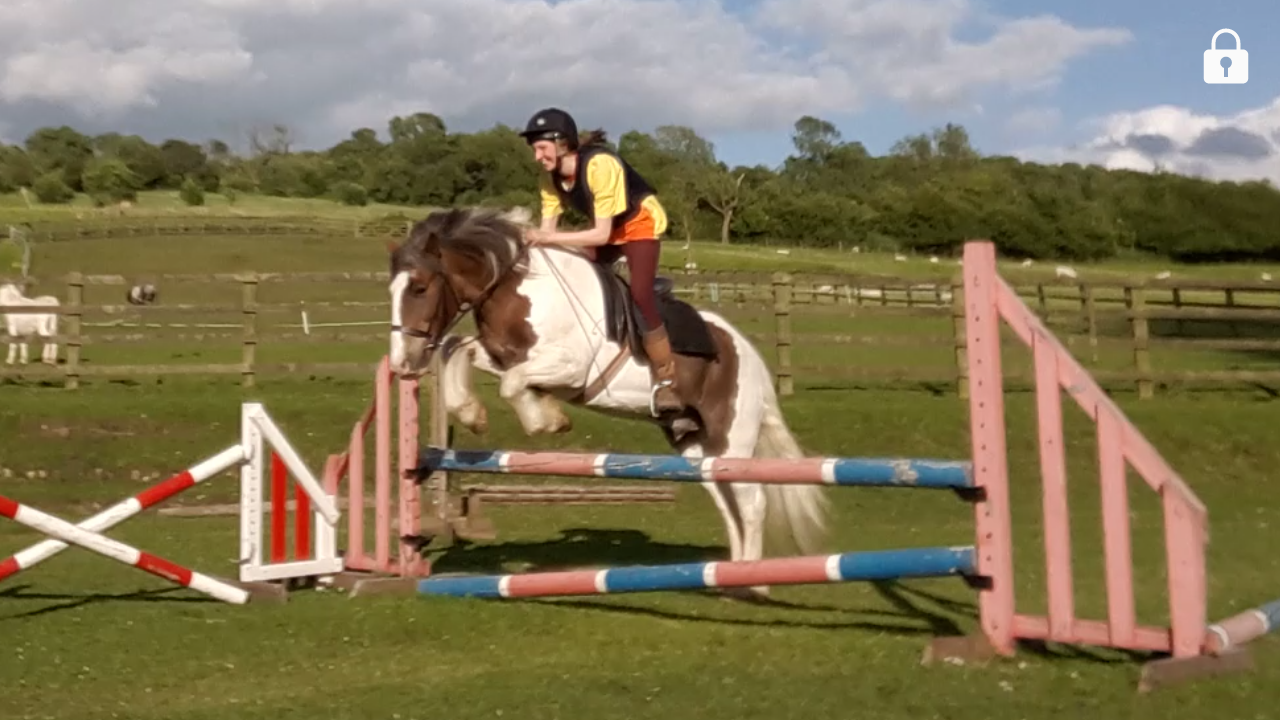
\includegraphics[width=\textwidth]{Figures/Harry}
\caption{Haribo}
\label{fig:plasma_source}
\end{figure}

\subsection{Effects of LTP on Wound Healing}

\begin{itemize}
\item Determining ox stress levels - markers for oxidative stress and how to measure them. Death, normal stuff RNA stuff?
\item Determining wound healing promotion - scratch test and if time allows, a 3D skin model, e.g. MatTek EpiDerm FT.
\item Draw a graph that has extent of ox stress and healing promotion on y axes, and changing plasma property on x axis
\item In the future, would be good to repeat this with bacteria, to see if the effects are similar
\end{itemize}




\subsubsection{Human Skin and the Healing Response}

The skin has three layers.
From superficial to deep, these are the epidermis, the dermis and the hypodermis, each of which have a different cellular composition and function as follows: \todo{Check where immune cells hang out...}
\begin{itemize}
\item The epidermis is made up of keratinocytes and is split from the dermis by a basement membrane. On the basement membrane, there are basal cells which produce the keratinocytes, melanocytes and sensory cells. Keratinocytes then move upwards from the basal layer, begin to produce keratin and then die. The surface of skin is, therefore, dead keratinocytes and keratin, which gives a waterproof barrier, and is sloughed off over time, to allow new keratinocytes up to the surface \toref{A skin paper!}
\item Dermis is composed of dense, irregular connective tissues, sweat glands, hair follicles and blood vessels \toref{}
\item Hypodermis consists mainly of loose connective tissue and fatty tissue \toref{}
\end{itemize}

Following wounding, the skin commences a well-defined healing phases: (1) coagulation and haemostasis, (2) inflammation, (3) proliferation and re-epithelialisation, and (4) wound remodelling \cite{Velnar2009the}.
Evidence suggests that RONS such as NO \cite{Shekhter2005beneficial}, and electric fields \cite{Thakral2013electrical, Messerli2011extracellular} have beneficial effects on the wound healing process, therefore, these are proposed mechanisms for the acceleration in wound healing seen by LTP treatment.
For more detail, please refer to my 6 month TAP report.


%The skin has different layers. The following information about skin layers comes from: 
%
%\url{https://opentextbc.ca/anatomyandphysiology/chapter/5-1-layers-of-the-skin/}
%
%
%There is the epidermis, the dermis and the hypodermis.
%The epidermis it the most superficial layer, exposed to the environment, and is composed almost entirely of keratin-producing cells, keratinocytes.
%The epidermis is made up of different layers, namely from deep to superficial, the stratum basale, stratum spinosum, stratum granulosum and stratum corneum.
%All except the stratum basale is made of keratinocytes, whereas the stratum basale consists mainly of basal cells (which are keratinocyte precurosrs), but also contains Merkel cells (touch receptors) and melanocytes (melanin-producing cells).
%As basal cells divide and produce daughter keratinocytes, the keratinocytes are pushed up through the epidermal layers, producing increasing amounts of keratin and then dying, leaving begin the keratin and cell membranes, so that the most superficial layer consists only of dead keratinocytes and their keratin.
%The epidermis also contains Langerhan's cells, which are a skin-specific dendritic cell, which is able to phagocytose invading pathogens and debris.
%
%The dermis is below the epidermis and contains structures such as blood vessels, hair follicles and sweat glands, in dense, irregular connective tissue.
%Finally, the hypodermis consists mainly of loose connective tissue and fatty tissue.
%
%A real paper on skin structure \cite{Mancini2014microRNAs}...
%
%When considering wound treatments using LTP, depending on the type and severity of the wound, the skin cells that will be exposed will vary.
%However, since keratinocytes form the bulk of the epidermis, it is reasonable to start any investigations of LTP effects on skin cells in these cells.

\subsubsection{Aims of Biology Experiments}

For the time being, I have decided to focus my project on the wound healing promotion aspect of wound treatments, as opposed to bacterial killing.
This is particularly important for determining the safety of LTP treatment, as well as looking into the beneficial effects induced by plasma on wound healing.
To begin with, cell lines will be used, for example, keratinocyte cell lines. 
However, if time allows, then the project will hopefully be able to progress into using a more advanced model for wound healing, such as the EpiDerm FT model from MatTek Corporation \cite{MattekWebsite}, which is a fully stratified, full thickness skin model, which has been used previously for wound healing investigations.

The aims of the biology arm of this project are as follows:
\begin{enumerate}
\item Decide on a suitable end point for measurement following LTP treatment. In particular, I am interested in the oxidative stress induced in skin cells following LTP treatment, and in measuring factors that are up/downregulated for successful wound healing and how they are affected by LTP treatment.
\item Develop a suitable experiment that is easily reproducible so can be repeated many times for different types of plasma treatment. As the overall aim of the biology is to look at how different plasma compositions can affect biological outcomes, it is important to have an experiment that can be repeated many times and be robust enough to give consistently measurable, quantitative results.
\item Determine how different plasma treatments can affect the biology outcomes
\end{enumerate}

In particular, it will be of interest to look at the differential effects of LTP treatment on both healthy skin/skin cells, as well as the "wounded" skin cells immediately at the wound edge.
This is because, even though they are the same cell type, their immediate environment will be very different.
A diagram of this concept is shown in \textbf{figure \ref{fig:wound_diagram}}.

\begin{figure}
\centering
\includegraphics[width=0.5\textwidth]{Figures/wound_diagram}
\caption{A wound...}
\label{fig:wound_diagram}
\end{figure}

\subsubsection{Detection of Oxidative Stress in Skin Cells}

At low levels, RONS are highly important for normal physiological cell function \cite{Fang2004antimicrobial, Thannickal2000reactive}.
However, if the concentration of RONS rises excessively for cells, then they can have toxic effects, for example, causing protein damage \cite{PhamHuy2008free}, lipid peroxidation \cite{Ayala2014lipid} and DNA damage \cite{Dizdaroglu2012oxidatively}, leading ultimately to cell death.

In order to detect oxidative stress induced by plasma treatment, a suitable end point to measure needs to be determined.
It seems that there are at least three ways to go about this, as follows:
\begin{enumerate}
\item Monitoring cell death.
This is a very nonspecific measurement, though it gives a rough overall picture of how damaging a treatment is, looking at the percentage of a cell population that can survive.
\item Measuring products of RONS attack.
For example, lipid peroxidation products such as malondialdehyde (MDA) and 4-hydroxynonenal (4-HNE) \cite{Ayala2014lipid} and DNA damage products such as \todo{DNA product - 8-OHdG????}. To do this, fluorescent probes could be used \cite{Ayala2014lipid, Joshi2011nonthermal, Joshi2010control} \todo{Quantitiative??}
\item Measuring an endpoint at the DNA/RNA/miRNA/gene expression level. Speak to Dmitris.
%miRNA in wound healing \cite{Riemondy2014not} - a review suggests wound healing promoted by miR-99 downregulation, and others may also be involved in wound healing. Downregulation of miR-199a-5p and miR-200b supports angiogenesis.
%miR-200c is involved in wound healing. Downregulation is required for proper healing as upregulation inhibits cell migration during wound repair  \cite{Aunin2017exploring}. 
%miR-200c is also upregulated by oxidative stress \cite{Magenta2011miR}. Yay.
%miR-25??
\end{enumerate}





%Oxidative stress is when cells/tissues are overwhelmed by oxidants. 
%Oxidants are things which cause oxidation.
%Free radical chain reactions normally produce numerous non-radical oxidants, such as hydrogen peroxide \toref{reference: https://hstalks.com/t/374/introduction-to-free-radicals-and-the-oxygen-parad/?biosci} .
%
%Oxidative stress can lead to induction of lipid peroxidation and modulation in the levels of antioxidant and drug-metabolising enzymes.
%ROS have also been demonstrated to induce some transcription factors, such as activating protein 1 (AP-1), and NF-$\kappa$B. 
%UVA is also involved in NF-$\kappa$B activation.
%Mitogen-activated protein kinase (MAPK) pathway is also a target of oxidative stress \cite{Bickers2006oxidative}.
%
%\cite{Nadal2011controlling} - paper talking about different sensors/transduction mechanisms/effectors but mainly in yeast and drosophilia
%
%\cite{Bickers2006oxidative} - another paper talking specifically about the skin and the role of oxidative stress in disease
%
%Kim2005role - something to do with MAPK in mouse skin following heat treatment
%
%Escuin-Ordinas2016cutaneous - something to do with MAPK, ERK and wound healing!





\subsubsection{Quantifying Wound Healing Promotion}

\begin{itemize}
\item Need a skin model - MatTek EpiDerm FT \cite{MattekWebsite} is a possibility. They have done wound healing assays before, cool ones using fluorescence etc.
\item Simple scratch assay - monolayer of keratinocytes in a petri dish, scratch then and see how long it takes for them to re-grow to confluence. Could be interesting to look at different things alongside this. Ie, have two plates scratched identically - watch one regrow and take the other to look at gene/miRNA expression/oxidative stress/markers of wound healing. Type of keratinocyte changes on activation \cite{Pastar2014epithelialization} and transcription factor induction (e.g. slug \cite{Savagner2005developmental}).
\item Do keratinocytes need to be wounded to be able to induce the wound healing promotion?! Or is the role of oxidative stress different in wounded and healthy keratinocytes?? \textbf{Figure \ref{fig:wound_diagram}}
\end{itemize}

\subsection{COST jet comparison}

COST microplasma jets are designed to be reference plasma sources that behave comparably, with a particular focus on biomedical applications \cite{Golda2016concepts}.
Recently 4 jets have been compared in the lab, in terms of power, temperature and optical emission.
The next step is to determine if all the jets also have comparable abilities to kill bacteria.
To investigate this, E.coli MG1655 on agar plates will be exposed to the plasma jets and the area of the plates where bacteria has been killed will be analysed, the so-called killing zone.
This will be a good opportunity to work with bacteria and will help with my project.

%\begin{itemize}
%\item COST microplasma jets are designed to be reference jets, for biomedical applications \todo{Check if for bio stuff}
%\item Have 4 jets being compared in the lab. So far all compare well in terms of power, temperature and emission. Now want to check biology interactions
%\item Aim is to determine whether they al have equivalent ability to kill bacteria, therefore the killing zone of each of the jets will be determined, by treating agar plates of E.coli MG1655 with each jet, then the kill zone established.
%\item Bacteria will be grown, then plated onto agar plates, before being exposed to the plasma jet. 
%The plates will then be incubated, and colonies counted and pictures taken, to determine the extent of the area of bacteria that has been killed by the plasma.
%\end{itemize}
 

\section{Immediate Plans}


\begin{itemize}
\item Learn to culture bacteria for COST comparison
\item Learnt to culture keratinocytes
\item Decide on biology experiment end points (e.g. oxidative stress, wound healing markers etc). Speak to the relevant experts e.g. Dmitris Lagos for miRNA
\end{itemize}

\section{Project Outlook}

















%\section{Oxidative Stress}
%Oxygen derived species - $\cdot$OH, O$_2^-\cdot$ and H$_2$O$_2$. However, O$_2^-\cdot$ and H$_2$O$_2$ have a low chemical reactivity, and do not readily react with biological molecules such as DNA, proteins and lipids. On the other hand, $\cdot$OH is very highly reactive, with reaction rates at or near diffusion-controlled rates for reactions with DNA \cite{Dizdaroglu2012oxidatively}.
%
%\subsection{DNA Damage}
%
%
%\section{Detecting Oxidative Stress - Bacteria}
%Different ways of detecting oxidative stress in bactera.
%In general, things to look for are cell death, membrane damage, DNA damage, lipid peroxidation and functional changes in proteins (e.g. enzyme deactivation).
%
%\subsection{Cell death}
%Measuring cell death can be done by measuring population level cell death, e.g through looking at zones of inhibition etc or at cellular level, e.g. using exclusion dyes.
%
%\subsection{Lipid Peroxidation}
%\begin{itemize}
%\item Lipid - large molecules made from smaller units of fatty acids and glycerol 
%\item Fatty acid - carboxylic acid consisting of a hydrocarbon chain and a terminal carboxyl group.
%\end{itemize}
%
%Radicals can attack polyunsaturated fatty acids and initiate lipid peroxidation in membranes.
%This can have significant effects on membrane fluidity and membrane-bound proteins.
%As a result of lipid peroxidation, aldehydes are often formed, which are long lived and able to function as "toxic second messenger" molecules, which can cause further damage to cells, in particular proteins \cite{Cabiscol2000oxidative}.
%These products include malonaldehyde (MDA) and 4-hydroxynonenal (HNE), which are particularly mutagenic and toxic, respectively \cite{Ayala2014lipid}.
%
%\subsection{DNA damage}
%
%\section{Methods}
%
%\begin{itemize}
%\item XTT assay. Metabolic activity
%
%Paper talking about oxidative stress in bacteria \cite{Cabiscol2000oxidative}. Talks about attack on lipids, proteins and DNA.
%
%\cite{Ezraty2017oxidative} is a paper with lots of biochemistry-y stuff in. Haven't read it - think it is a bit too in depth all about the mechanisms of protein damage, in particular sulphur containing side chains of proteins.
%
%\cite{Alkawareek2014potential} Paper looked at LTP interactions with bacteria, in particular bacterial killing/metabolism XTT assay (E. Coli, P. aeruginosa, B. cereus and MRSA), plasmid DNA damage (single and double strand breaks by looking whether the plasma was supercoiled (undamaged), open circular (single strand break) or linear (double strand break)), protein function (proteinase K's function was watched to see if the plasma was altering the structure in some way to prevent catalytic activity (it is pretty robust to changes in temp and pH therefore decrease in activity likely to be due to structural changes)), lipid peroxidation (MDA measurement in E. Coli) and membrane permeability (by measuring ATP leakage from E. Coli).
%\end{itemize}
%
%Assays:
%\begin{enumerate}
%\item \url{https://www.caymanchem.com/product/589320} - DNA/RNA Oxidative Damage ELISA Kit. Looks for 8-hydroxy-2'-deoxyguanosine from DNA, 8-hydroxyguanosine from RNA, and 8-hydroxyguanine from either DNA or RNA.
%\item
%\end{enumerate}
%%\section{}
%%\subsection{}
%
%\section{Detecting Oxidative Stress - Skin Cells}
%
%
%
%\section{Skin Models for Wound Healing Assays}
%Skin explants (people) can be cultured (as an organ culture) for up to 2 weeks at the air/liquid interface \cite{Gottrup2000models}.
%\subsection{Porcine Skin}
%
%\subsection{Hyaluronic Acid}
%
%\section{Cancer Things}
%\subsection{Radiotherapy}
%Radiation therapy can either be photon or particle, radiation.
%Photon radiation uses gamma ray or x ray beams focussed on the tumour, whereas particle radiation uses electrons, neutrons or protons for the same purpose - energy deposition into the tumour.
%By targeting the tumour with these beams, they deposit energy in the tumour cells, and cause ionisation of particles in the cells.
%This then leads to radical formation etc which causes damage to cancer cell DNA and prohibits their replication.
%Healthy cells are generally better at repairing DNA defects, meaning that if doses are delivered that cause sub-lethal levels of damage to healthy cells, then the healthy cells have time to repair before the next dose (as they divide much more slowly than cancer cells, so have longer to repair damage), whereas, cancer cells don't and therefore die.
%This gives specificity of a fashion.
%Damage to DNA occurs both directly (ie, the radiation directly damages the DNA), or indirectly, through formation of radical species which then attack the DNA. \cite{Baskar2012cancer}
%
%
%\subsection{Immunotherapy}
%\subsection{Photodynamic therapy}



\scriptsize
\bibliographystyle{ieeetr}
\bibliography{/Users/hld523/Bibliography/MyPapers}
\end{document}  